%%=============================================================================
%% Methodologie
%%=============================================================================

\chapter{\IfLanguageName{dutch}{Methodologie}{Methodology}}
\label{ch:methodologie}

%% TODO: Hoe ben je te werk gegaan? Verdeel je onderzoek in grote fasen, en
%% licht in elke fase toe welke stappen je gevolgd hebt. Verantwoord waarom je
%% op deze manier te werk gegaan bent. Je moet kunnen aantonen dat je de best
%% mogelijke manier toegepast hebt om een antwoord te vinden op de
%% onderzoeksvraag.



Na de stand van zaken die gebaseerd is op de literatuurstudie volgt de volgorde van stappen die ondernomen zijn om deze proef te voltooien. 

\section{z/OS Health Checker standaard setup}
\label{sec:z/OS Health Checker Standaard setup}

De eerste onderzoeksvraag was of er een mogelijkheid was tot een standaardopstelling binnen de z/OS Health Checker omgeving van HCL Technologies. Maar eerst moet er een analyse plaatsvinden op de huidige opstelling van Health Checker zodat we die kunnen optimaliseren.

\subsection{Analyse van huidige z/OS Health Checker Setup}
\label{subsec:Analyse van huidige z/OS Health Checker Setup}
De opstelling die in deze proef geanalyseerd werd bevindt zich binnen een parallel sysplex. En deze parallel sysplex werken we met 4 LPARS: VT1, VT2, VT3 en VT4. Elke LPAR heeft verschillende checks. Maar na de 4 LPARS te overlopen was het duidelijk dat de meeste checks op VT1 draaien. Daarom ligt de focus van de analyse op VT1.

De analyse is gemaakt met de check data uit SDSF. Deze kan je bereiken door bij het ISPF hoofdmenu volgende optie te geven 's;ck'. Dit is S voor SDSF met als optie CK voor Health Checker(zie figuur \ref{fig:sdsfck}).

\begin{figure}[h]
	\centering
	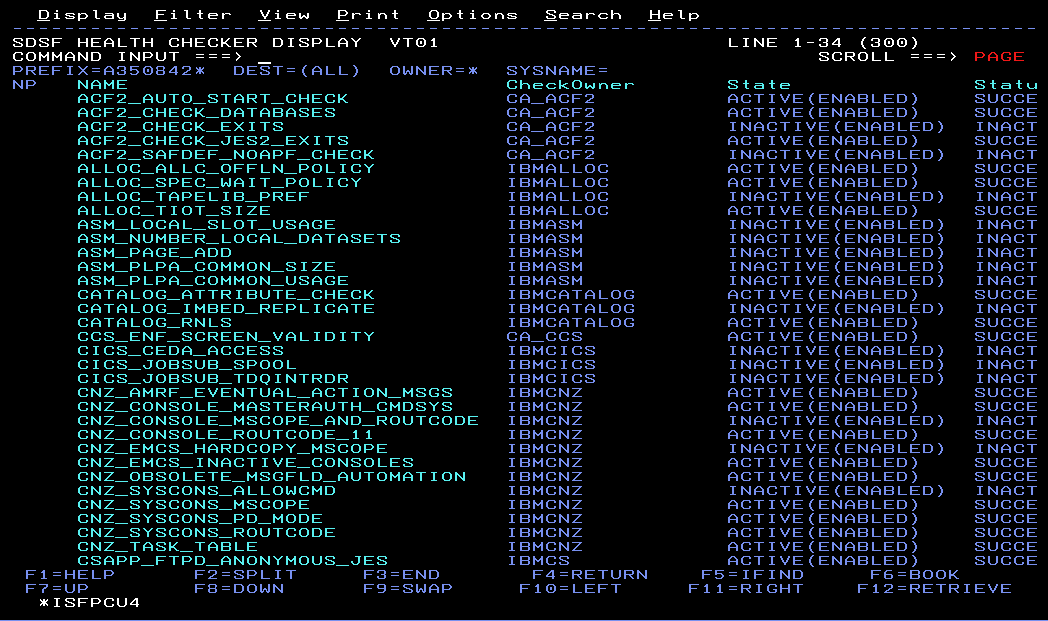
\includegraphics[width=0.7\linewidth]{img/SDSFCK}
	\caption[Health Checker Scherm binnen SDSF]{{\small \textit{Dit is het Health Checker paneel binnen SDSF hier kunnen we de output zien van de laatste keren dat een check is uitgevoerd}}}
	\label{fig:sdsfck}
\end{figure}


Na het overlopen van alle checks op VT1 hebben we de SDSF output samengevat in volgende tabel. Deze tabel bevat volgende eigenschappen van een check.

\begin{itemize}
	\item De naam van de check.
	\item De status, deze beschrijft of de check aanstaat of niet.
	\item De outcome, deze beschrijft of de check succesvol was of niet.
	\item De reason, dit is de reden waarvoor de check draait.
\end{itemize}

Een voorbeeld:

\begin{table}[]
	\begin{tabular}{|p{5cm}|p{3.5cm}|p{1.5cm}|p{5cm}|}
		\hline
		\textbf{Name} & \textbf{Status} & \textbf{Outcome} & \textbf{Reason} \\
		\hline
		XCF\_CDS\_MAXSYSTEM & ACTIVE(ENABLED) & SUCCES & CDS MAXSYSTEM value across all CDS types should be at least equal to the value 
		in the primary sysplex CDS.  \\
		\hline
	\end{tabular}
	\caption[Individuele check]{{\small \textit{Waarden van de check die bij de eerste analyse werden samengevat}}}
	\label{tbl:Individuele check}
\end{table}


Voor de volledige tabel zie bijlage \ref{sec:Tabellen Standaard opstelling z/OS Health Checker} 

Hier uit bleek dat er verscheidene checks een exception hadden. Deze zijn eerst gecontroleerd om te zien dat men deze zelf kon oplossen zonder ondersteuning van de collega's die het product beheren. Bij deze analyse bleek ook dat er veel checks zijn die onnodig draaiden omdat het product van de check bijvoorbeeld niet aanwezig was. Niet alle checks moeten in alle LPARs draaien en sommige moesten aangepast worden. Maar daarvoor heb je nog de belangrijke vraag of een wijziging van een check doorgevoerd moet worden naar alle LPARs of maar naar 1 LPAR binnen de Parallel Sysplex. Met deze informatie is naar feedback gevraagd van alle Mainframe Teams binnen HCL Technologies. Zonder deze feedback van het verantwoordelijke team kan je de checks niet aanpassen Hiervoor zijn alle checks gegroepeerd per owner en per mainframe team zodat we uiteindelijk tot tabel \ref{tbl:Checks Per Team} komen. Deze tabellen zijn er gekomen na veel overleg om zo tot de beste setup te bekomen.

Nog een kleine verduidelijking voor alle teams die belang hebben bij de z/OS Health Checker setup.
\begin{itemize}
	\item CICS: Dit team is verantwoordelijk voor de IBM CICS Software\footnote{Customer Information Control System dit is software voor het verwerken van transacties (\cite{ChrisRayns2011}) }
	\item Communication: Dit team is verantwoordelijk voor alle communicatie-gerelateerde software zoals TCP/IP, FTP\footnote{File Transfer Protocol}, etc.
	\item Print: Dit team is verantwoordelijk voor alle output software zoals CA-View\footnote{Tool van Computer Associates}, VPS, etc.
	\item Automation: Dit team is verantwoordelijk voor alles wat met automatisering te maken heeft. Vooral software zoals System Automation, NetView en GDPS. Dit team is het meest betrokken bij monitoring.
	\item ROO: Roll-Out \& Operate, dit team beheert de 'basics' van z/OS. Dit team voert ook de upgrades uit.
	\item RTC: RunTime Control, dit team is verantwoordelijk voor performance en rapportering.
	\item Security: Security: Dit team spreekt voor zich. Het beheert tools zoals RACF/ACF2/Top Secret dit zijn allemaal tools die extra beveiliging aanbieden voor de mainframe.	
	\item SOE: Standard Operating Environment, dit team doet alle installaties van software voor de mainframe.
	\item Storage: Dit team beheert alles wat te maken heeft met opslag en ook de software die erbij hoort.
	\item zOPEN: Dit team beheert alles van zLinux\footnote{Een linux besturingsysteem voor mainframe} samen met Unix System Services\footnote{UNIX besturingssysteem implementatie voor de mainframe} en Websphere\footnote{Software product gericht op web-technologie}
	\item DB: Database team, beheert alle database systemen waaronder DB2.
\end{itemize}

Alle Check owners gegroepeerd per team.

\begin{table}[h]
	\begin{tabular}{|l|p{9cm}|}
		\hline
		\textbf{Team}                      & \textbf{Checks(Owner)}                                                                                                                                                 \\ \hline
		\textbf{Cics}                      & IBMCICS                                                                                                                                                                \\ \hline
		\textbf{Communication}             & IBMCS, CA\_TPX                                                                                                                                                         \\ \hline
		\textbf{Print}                     & CA\_DLVR, CA\_SPOOL, CA\_VIEW                                                                                                                                          \\ \hline
		\textbf{Rollout and Opperate(ROO)} & CA\_CSS, IBMCNZ,  IMBCTRACE, IBMDAE, IBMISPF, IBMXLOGR, IBMJES(2), IBMRRS, IBMRTM, IBMSDSF, IBMSDUMP, IBMSLIP, IBMSVA, IBMSYSTRACE, IBMTIMER, IBMTSOE,  IBMXCF, IBMGRS \\ \hline
		\textbf{Run Time Control(RTC)}     & IBMVLF, CA\_PMO, IBMRCF, IBMASM, IBMRSM, IBMSUP, IBMVSM,  CPWR\_THRUPUT\_MGR                                                                                           \\ \hline
		\textbf{Security}                  & CA\_ACF2, IBMICSF                                                                                                                                                      \\ \hline
		\textbf{SOE}                       & All checks starting with ZOSMIG                                                                                                                                        \\ \hline
		\textbf{Storage}                   & CA\_DISK, IBMALLOC, IBMCATALOG, IBMDMO, IBMHSM, IMBIOS, IBMOCE, IMBPDSE, IBMSMS, IBMVSAM(RLS), CA\_VANTAGE                                                             \\ \hline
		\textbf{zOpen}                     & IBMSSH, IBMUSS, IBMZFS                                                                                                                                                 \\ \hline
		\textbf{Databse(DB)}               & CA\_DB2, CA\_DTCM, CA\_IDMS                                                                                                                                            \\ \hline
		\textbf{Automation}                & IBMGDPS                                                                                                                                                                \\ \hline
	\end{tabular}
	\caption[Checks Per team]{{\small \textit{Alle checkowners gegroepeerd per team binnen HCL}}}
	\label{tbl:Checks Per Team}
\end{table}

Nadat alle checks per team werden gegroepeerd, is er eerst zelf een voorstel gemaakt voor de opstelling van hun checks waar zij feedback op konden geven. Wanneer er geen feedback was is de voorgestelde opstelling geïmplementeerd. Als een check gewijzigd wordt moet dit gedefinieerd worden in de parmlib. Maar men moet ook weten of een wijziging in alle LPARs moet gebeuren of maar in 1 LPAR. Daarom hebben we bij de tabellen van de gehele setup nog 2 extra kolommen.

\begin{itemize}
	\item Run: Dit definieert dat de check uitgevoerd moet worden(Yes of No). Of dat deze check aangepast moet worden(MOD).
	\item 00/\&SUF: Dit definieert dat de check voor alle LPARs wordt uitgeschakeld (00) of maar voor 1 LPAR(\&SUF\footnote{Dit is een omgevings variabele dat de huidige LPAR specifieerd}). Wanneer er N/A(not applicable) staat betekent dit dat er niets verandert zal worden aan de check.
\end{itemize}

Verder was er nog 1 uitzondering voor het beheren van de checks. Het SOE team beheert alle migratie checks en deze zullen ongewijzigd blijven in de parmlibs. De migratie checks zelf worden maar 1 keer geactiveerd.

De volledige health Checker setup zoals ze na deze proef is bevindt zich in bijlage \ref{sec:Tabellen Standaard opstelling z/OS Health Checker}. Dit is een samenvatting van hoe HCL wilt dat de setup eruit ziet. 

\subsection{Parmlib Members voor de standaard setup}
\label{subsec:Parmlib Members voor de standaard setup}

Om dit door te voeren moeten we de parmlib members wijzigen. Als een check over het gehele systeem wordt uitgeschakeld gebeurt dit in HZSPRM00. Is het voor een enkele LPAR dan moet de wijziging gedefinieerd worden in de parmlib member van die LPAR. Er zijn 5 parmlib members voor z/OS Health Checker binnen de setup van HCL Technologies.

\begin{enumerate}
	\item HZSPRM00: Wijzigingen in deze member gelden voor alle LPARs binnen de parallel sysplex.
	\item HZSPRMT1: Wijzigingen in deze member gelden enkel voor VT1
	\item HZSPRMT2: Wijzigingen in deze member gelden enkel voor VT2
	\item HZSPRMT3: Wijzigingen in deze member gelden enkel voor VT3
	\item HZSPRMT4: Wijzigingen in deze member gelden enkel voor VT4
\end{enumerate}

Deze wijzigingen gebeuren met een ADDREPLACE-statement. Het statement in figuur \ref{fig:addreplace} doet het volgende:

\begin{itemize}
	\item Statement(NOPLEX) specificeert de naam van de wijziging
	\item Update specificeert dat de check zal blijven draaien maar met andere parameters. Dit kan ook 'inactive' zijn om de check te deactiveren of 'Delete' om de check te verwijderen.
	\item Check(,) definieert de check owner en de check zelf die gewijzigd wordt.
	\item Parm('NOPLEX') dit is de parameter die meegegeven wordt voor de wijziging.
	\item Reason() dit is een zelf in te vullen reden voor het wijzigen van de check.
	\item Date(20090701) dit is de datum van de wijziging in yyyymmdd formaat. \cite{Bezzi2010}
\end{itemize}

\begin{figure}[h]
	\centering
	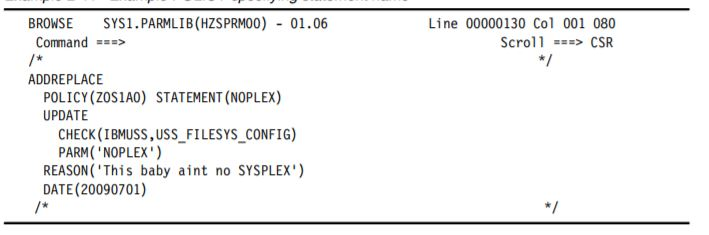
\includegraphics{img/addreplace}
	\caption[ADDREPLACE statement]{{\small \textit{Voorbeeld van een ADDREPLACE Statement (\cite{IBMCorporation2019})}}}
	\label{fig:addreplace}
\end{figure}

Bij de analyse van de setup bleek ook dat er veel checks waren die de GLOBAL status hadden. Maar deze draaiden verspreid over de 4 LPARs. Voor de nieuwe standaard setup van z/OS Health Checker wenste HCL Technologies dat alle GLOBAL checks draaide op de VT1 LPAR, hiervoor moesten dus alle GLOBAL checks inactief gezet worden op alle LPARs buiten VT1. Dit is mogelijk door dat te doen in volgende parmlib members: HZSPRMT2, HZSPRMT3 en HZSPRMT4. Met deze requirements zijn de 4 parmlib members aangemaakt. Deze bevinden zich in bijlage \ref{sec:Parmlin members voor z/OS Health Checker}

Nadat de parmlib members aangepast werden, moeten ze nog door het systeem geïmplementeerd worden. Dit doet men met volgende commando's in SDSF.

\begin{itemize}
	\item /F HZSCHK,REPLACE,PARMLIB=(00,T1) voor LPAR VT1. 
	\item /F HZSCHK,REPLACE,PARMLIB=(00,T2) voor LPAR VT2.
	\item /F HZSCHK,REPLACE,PARMLIB=(00,T3) voor LPAR VT3.
	\item /F HZSCHK,REPLACE,PARMLIB=(00,T4) voor LPAR VT4.
\end{itemize}

Verder is er nu ook een HSPRMTK member. Dit is een kopie van HZSPRMT4. Als het syteem zou uitbreiden met een LPAR, zal deze member gebruikt worden om z/OS Health checker in te stellen voor de nieuwe LPAR. de HZSPRMT4 member is gekozen omdat deze het meest geschikt is voor nieuwe LPARs.

\section{Logging van z/OS Health Checker}
\label{sec:Logging van z/OS Health Checker}

Nu er een standaard setup van z/OS Health Checker tot stand is gekomen, is er nog een een systeem nodig dat de potentiële problemen kan loggen. Want SDSF zal geen berichten sturen naar gebruikers dat er een probleem is. Via SDSF zal je enkel zelf kunnen kijken tussen alle checks om te zoeken welke een exception hebben. Daarom zijn er JCL jobs geschreven, die voor elke LPAR een mail gaan sturen met alle checks die in exception staan. Deze mail gaat naar een team in India dat ervoor zal zorgen dat de problemen opgelost worden. Omdat checks meerdere keren draaien zal er met IBM Tivoli Workload scheduler een plan gemaakt worden. Met dit plan zullen de jobs automatisch elke vrijdag draaien.

\subsection{JCL jobs voor het logging}
\label{subsec:JCL jobs voor het logging}
De jobs zelf bevinden zich in bijlage \ref{sec:JCL jobs}. De JCL job in bijlage \ref{subsec:FHZSVT11} zal gebruikt worden om de werking van de job uit te leggen.

De eerste regels van de job definiëren zijn naam en zijn eigenschappen. Deze job wordt dan gebonden aan VT01 omdat hij voor deze LPAR draait.

\fbox{
	\parbox{\textwidth}{
		//FHZSVT11 JOB (610VV110000,4352,,,,1800),'RTN=FHZSPRVT',CLASS=D,  \\ 
		//          MSGCLASS=A,MSGLEVEL=(1,1)                              \\ 
		/*ROUTE XEQ NJEVT                                                  \\
		/*ROUTE PRINT NJOVT                                                \\ 
		//*+JBS BIND VT01                                                  \\ 
		//*    															   
	}
}

Dan wordt het HZSPRINT programma opgeroepen. Met de parameters zoals hieronder, roep je alle checks aan van alle owners met een exception. Er worden hier voor wildcards gebruikt(*). 

\fbox{
	\parbox{\textwidth}{
		//HZSPRINT EXEC PGM=HZSPRNT,     \\                                   
		//   PARM='CHECK(*,*),EXCEPTIONS'          							   
	}
}     

De output van het HZSPRINT prorgamma word in een tijdelijk bestand gestopt als volgt.

\fbox{
	\parbox{\textwidth}{
	//SYSOUT   DD DISP=(NEW,PASS),DSN=\&\&OUT,LRECL=256,RECFM=FB,         \\
	//         DATACLAS=PSEN                                              \\
	//*    							   
	}
}     

Dan wordt er met het SMTPAPIX programma een mail opgezet via noreply@volvo.com.Deze gebruikt het tijdelijke bestand als input(MEMO statement), dit bestand wordt dan verzonden naar de email adressen waarnaar verwezen wordt in de job.

\fbox{
	\parbox{\textwidth}{
		//SNDMEM  EXEC PGM=SMTPAPIX,PARM='MSGLVL=4, \\
		//        FROM=NOREPLYÖVOLVO.COM', \\
		//             COND=(0400,EQ,HZSPRINT)                              \\
		//APIFILE DD *                                                      \\
		)SEND                                                               \\
		ETITLE    VT01: Health Checker exceptions                         
	}
}
\fbox{
	\parbox{\textwidth}{
		OPTION   FORCE  													\\	
		DEST     jonas.braemÖsupplier.volvo.com                          	\\
		DEST     david.westbrandÖhcl.com                                 	\\
		DEST     kevin.somersÖhcl.com                                    	\\
		DEST     bengt.gellingskogÖhcl.com                               	\\
		MEMO FILEA                                                       	\\
		)END 						   
	}
} 

Als laatste zal het tijdelijk bestand verwijderd worden met volgende code.

\fbox{
	\parbox{\textwidth}{
		//FILEA DD DISP=(OLD,DELETE),DSN=\&\&OUT						   
	}
}  

De mail zelf zal nu de check output bevatten van alle checks met een exception zoals in bijlage \ref{subsubsec:Check Output}

\subsection{Jobs schedulen met IWS}
\label{subsec:Jobs schedulen met IWS}

Eens de jobs klaar zijn moeten ze gepland worden. In de setup van HCL zullen de jobs elke vrijdag moeten draaien. Dit zal gebeuren met IBM Tivoli Workload Scheduler(IWS). Met deze tool kunnen we jobs automatisch laten uitvoeren met een interval. Je kan deze tool vergelijk met CRON op linux. Om de scheduler te initializeren wordt volgend commando gebruikt vanuit het ISPF hoofdmenu

\fbox{
	\parbox{\textwidth}{
		TSO OPCA
	}
} 

Hier is dan een plan opgesteld met de 4 print jobs als volgt. De FHZRS is een 'Routine start' en de FHZSRE een 'Routine exit' om zo het begin en einde van het plan af te
bakenen(zie figuur \ref{fig:iws}). 

\begin{figure}[h]
	\centering
	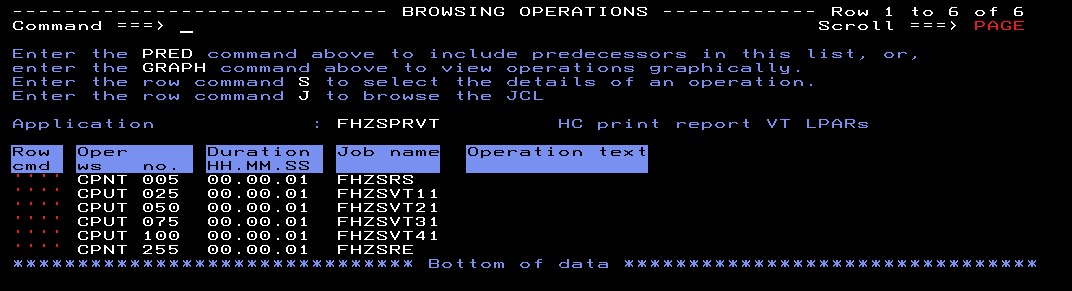
\includegraphics[width=1\linewidth]{img/IWS}
	\caption[Plan voor de print jobs]{{\small \textit{Het plan met de 4 JCL print jobs samen met een routine start en routine end.}}}
	\label{fig:iws}
\end{figure}

 Dan moet men het interval instellen dat bepaalt wanneer het plan uitgevoerd wordt. Dit moet elke vrijdag gebeuren. Dit stel je in als volgt(zie figuur \ref{fig:interval}).

\begin{figure}[h]
	\centering
	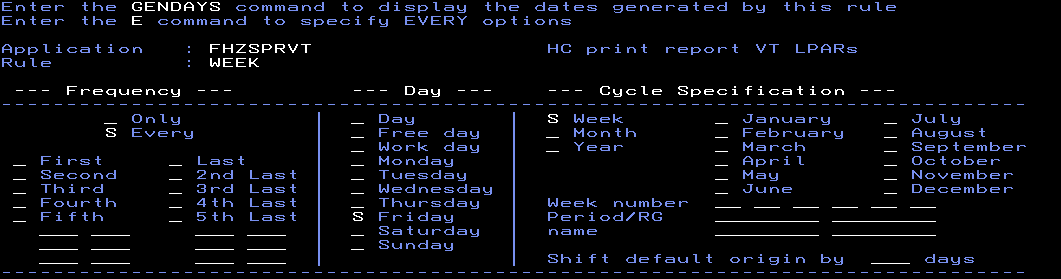
\includegraphics[width=1\linewidth]{img/Interval}
	\caption[Interval in IWS]{{\small \textit{Het interval is ingesteld om het plan elke vrijdag van elke week uit te voeren.}}}
	\label{fig:interval}
\end{figure}

Om na te kijken of het interval goed ingesteld is kunnen we via het GENDAYS commando via het scherm op figuur \ref{fig:interval} naar een kalender te gaan. Deze kalender duid alle dagen dat het plan zal uitvoeren aan in het blauw. En op figuur \ref{fig:calender} is te zien dat dit alle vrijdagen zijn vanaf 01/05/20. Dit is de datum wanneer het plan voor de eerste keer werd uitgevoerd. Dit plan staat gepland voor de komende 10 jaar zoals te zien is op figuur \ref{fig:caleder2030}

\begin{figure}[h]
	\centering
	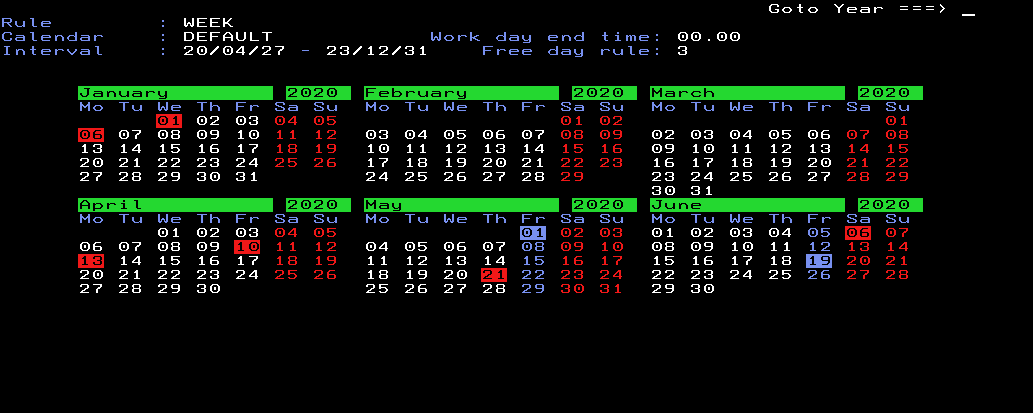
\includegraphics[width=0.8\linewidth]{img/Calender}
	\caption[Kalender IWS]{{\small \textit{De kalender duidt datums aan met een blauw lettertype. Op deze dagen zal het plan uitgevoerd worden}}}
	\label{fig:calender}
\end{figure}
\begin{figure}[h]
	\centering
	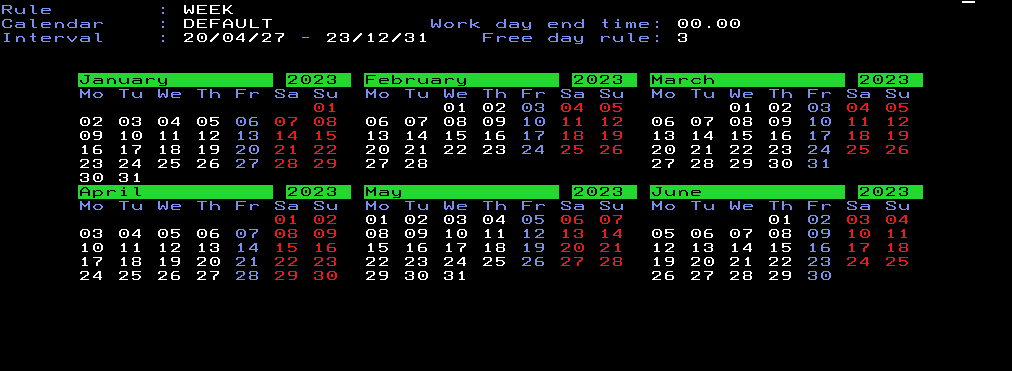
\includegraphics[width=0.8\linewidth]{img/Caleder2030}
	\caption[Kalender IWS 2030]{{\small \textit{Het interval van het plan staat alvast gepland tot 2031}}}
	\label{fig:caleder2030}
\end{figure}

Zoals te zien op de kalenders zijn de JCL jobs nu geprogrammeerd en zal een team elke vrijdag een log ontvangen met alle exceptions van alle LPARs. Het team zal dan de verantwoordelijke van de check met een exception aansporen om deze op te lossen. Door deze werking zal er nu efficiënter gewerkt worden met z/OS Health Checker en is er nog minder kans dat er problemen over het hoofd worden gezien.